In this section we will explore our findings from our research.

\subsection{Problem}
Consider a graph $G$ with edges $E$ and vertices $V$, and subgraphs $G_1, \ldots, G_k \subset G$. Let $G_i = (E_i, V_i)$ for these subgraphs. For now let us suppose the graph is unweighted and undirected. The subgraphs need not cover $G$ and can overlap. Each player $i$ knows $G$ and $G_i$, but not the other player's graphs. (This is akin to a map of a city, where each player is a different regional taxi company.) The goal is, given some starting vertex $v \in V$, and some end vertex, $w \in V$ to:
\begin{enumerate}
	\item  Identify if it is possible to construct a path $v, v_1, \dots, v_l, w$ such that every edge on the path is in $\bigcup_{i=0}^{k} E_i$. \label{one}
	\item  If such a path exists, find the minimum number of edges needed to get from $v$ to $w$, while using only edges belonging to $\bigcup_{i=0}^{k} E_i$. \label{two}
\end{enumerate}

\tikzset{
  point/.style={
    circle,
    fill,
    inner sep=1pt
  }
}

\begin{figure}[H]
\centering
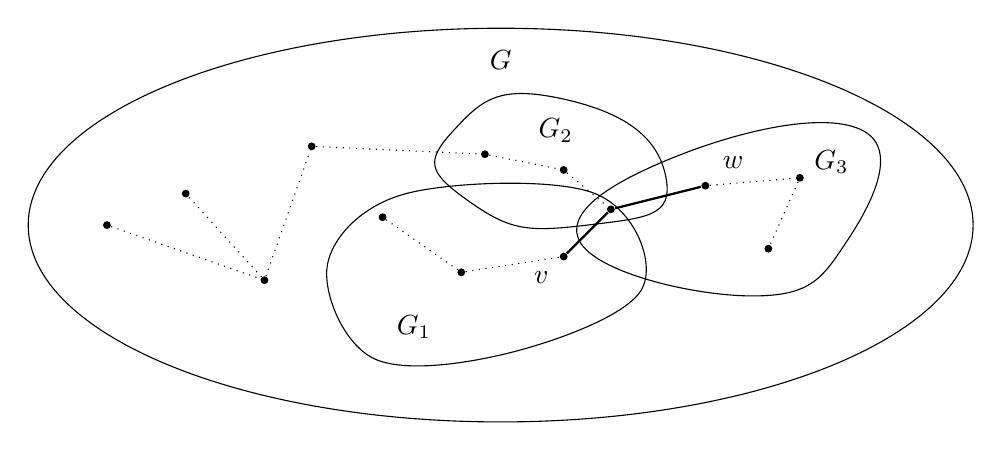
\begin{tikzpicture}
  \draw (0,0) ellipse [x radius=6, y radius=2.5];
  \node at (0,2.1) {$G$};

  \draw plot [smooth cycle, tension=0.6] coordinates {(-2.2,-0.5) (-1.2,0.4)
	  (1.2,0.4) (1.8,-0.8) (0.2,-1.6) (-1.6,-1.7) };
  \node at (-1.1,-1.3) {$G_1$};

  \draw plot [smooth cycle, tension=1.1] coordinates {(-0.6,1.2) (0.8,1.6)
	  (2.1,0.6) (1.1,0) (-0.4,0.3)};
  \node at (0.7,1.2) {$G_2$};

  \draw plot [smooth cycle, tension=0.8] coordinates {(2.3,0.9) (4.6,1.2)
	  (4.4,-0.2) (3.2,-0.9) (1.0,-0.2)};
  \node at (4.2,0.8) {$G_3$};

  \node[point] (a1) at (-1.5,0.1) {};
  \node[point] (a2) at (-0.5,-0.6) {};
  \node[point] (a3) at (0.8,-0.4) {};
  \draw[dotted] (a1) -- (a2) -- (a3);

  \node[point] (b1) at (-0.2,0.9) {};
  \node[point] (b2) at (0.8,0.7) {};
  \node[point] (b3) at (1.4,0.2) {};
  \draw[dotted] (b1) -- (b2) -- (b3);

  \node[point] (c1) at (2.6,0.5) {};
  \node[point] (c2) at (3.8,0.6) {};
  \node[point] (c3) at (3.4,-0.3) {};
  \draw[dotted] (c1) -- (c2) -- (c3);

  \node[point] (d1) at (-5,0) {};
  \node[point] (d2) at (-3,-0.7) {};
  \node[point] (d3) at (-2.4,1) {};
  \node[point] (d4) at (-4,0.4) {};
  \draw[dotted] (d1) -- (d2) -- (d4);
  \draw[dotted] (d2) -- (d3) -- (b1);

  \node[below left=0.1pt , outer sep=2pt] at (0.8,-0.4) {$v$};
  \node[above right=1pt , outer sep=2pt] at (2.6,0.5) {$w$};

  \draw[thick] (c1) -- (b3) -- (a3);
\end{tikzpicture}
\caption{A valid path from $v$ to $w$ in bold. Note that $G$ may contain nodes
not belonging to any player.}
\end{figure}

\subsection{Lower bound sketches and ideas}
For \cref{one}, we think this would require computing $\binom{k}{2}$ pairwise set disjointnes in the worst case, to determine where the intersections of each $G_i$ are, at which point each player could on their own determine the possible
paths between each of the subgraphs that intersect with their own. 

\begin{figure}[H]
\centering
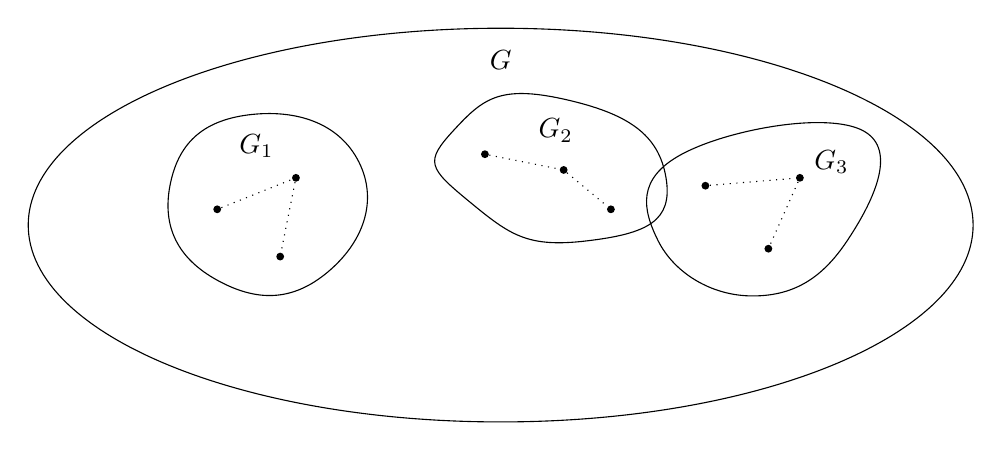
\begin{tikzpicture}
  \draw (0,0) ellipse [x radius=6, y radius=2.5];
  \node at (0,2.1) {$G$};

  \draw plot [smooth cycle, tension=0.9] coordinates {(-4.2,0.5) (-3.2,1.4) (-1.8,0.8) (-2.2,-0.6) (-3.6,-0.7)};
  \node at (-3.1,1) {$G_1$};

  \draw plot [smooth cycle, tension=1.1] coordinates {(-0.6,1.2) (0.8,1.6) (2.1,0.6) (1.1,-0.2) (-0.4,0.3)};
  \node at (0.7,1.2) {$G_2$};

  \draw plot [smooth cycle, tension=0.8] coordinates {(2.3,0.9) (4.6,1.2) (4.4,-0.2) (3.2,-0.9) (2.0,-0.2)};
  \node at (4.2,0.8) {$G_3$};

  \node[point] (a1) at (-3.6,0.2) {};
  \node[point] (a2) at (-2.6,0.6) {};
  \node[point] (a3) at (-2.8,-0.4) {};
  \draw[dotted] (a1) -- (a2) -- (a3);

  \node[point] (b1) at (-0.2,0.9) {};
  \node[point] (b2) at (0.8,0.7) {};
  \node[point] (b3) at (1.4,0.2) {};
  \draw[dotted] (b1) -- (b2) -- (b3);

  \node[point] (c1) at (2.6,0.5) {};
  \node[point] (c2) at (3.8,0.6) {};
  \node[point] (c3) at (3.4,-0.3) {};
  \draw[dotted] (c1) -- (c2) -- (c3);
\end{tikzpicture}
\caption{Worst case for \cref{one}: Disjoint Subsets}
\end{figure}


For \cref{two}, we would be required to compute $\binom{k}{2}$ pairwise
intersections, since in order to minimize the path we would need to know all
possible paths that could connect $v$ and $w$. To find the shortest path, each
player works backwards and sends the distances through their internal vertices
to the players they intersect with, and each player will attempt to identify if
a longer path can be dropped whenever they receive this list.



\subsection{Lower bound using Equality}

\paragraph{Equality problem.}
In the two-party Equality problem, Alice is given a string $x \in \{0,1\}^n$ and Bob is given a string $y \in \{0,1\}^n$. The goal is to determine whether $x = y$. It is known that Equality has deterministic communication complexity $\Omega(n)$.

\paragraph{Equality gadget.}
We construct a gadget that enforces equality at a single bit position. The gadget is shown in Figure~\ref{fig:equality_gadget}. The gadget consists of two parallel branches.

\begin{enumerate}
    \item The top branch corresponds to the assignment $x_i = y_i = 1$, 
    \item The bottom branch corresponds to the assignment $x_i = y_i = 0$. 
\end{enumerate}
 

\begin{figure}[h]
\centering
\begin{tikzpicture}[scale=1.2, every node/.style={circle, fill=black, inner sep=1.5pt}]

% Nodes

\node (L) at (-2,0) {};
\node (T1) at (-0.8,1.5) {};
\node (T2) at (0.8,1.5) {};
\node (B1) at (-0.8,-1.5) {};
\node (B2) at (0.8,-1.5) {};
\node (R) at (2,0) {};

% Edges
\draw (L) -- (T1);
\draw (T1) -- (T2);
\draw (T2) -- (R);

\draw (L) -- (B1);
\draw (B1) -- (B2);
\draw (B2) -- (R);

% Labels
\node[draw=none, fill=none, above=6pt] at (T1) {$x_i = 1$};
\node[draw=none, fill=none, above=6pt] at (T2) {$y_i = 1$};

\node[draw=none, fill=none, below=6pt] at (B1) {$x_i = 0$};
\node[draw=none, fill=none, below=6pt] at (B2) {$y_i = 0$};

\end{tikzpicture}
\caption{Gadget for proving equality. A path only exists if $x_i = y_i$ for either branch.}
\label{fig:equality_gadget}
\end{figure}


Alice enables exactly one entry node of the gadget depending on $x_i$, and Bob enables exactly one exit node depending on $y_i$. A path exists through the gadget if and only if Alice and Bob select nodes on the same branch, which holds exactly when $x_i = y_i$.\\

\paragraph{Reduction to our graph problem.}
We construct a graph by chaining one copy of this gadget for each index $i \in [n]$ between a global start vertex $v$ and end vertex $w$. In the resulting graph, there exists a path from $v$ to $w$ if and only if all gadgets are traversable, which occurs if and only if $x_i = y_i$ for all $i$, i.e., if and only if $x = y$.


\begin{figure}[h]
\centering
\begin{tikzpicture}[
hex/.style={
draw,
regular polygon,
regular polygon sides=6,
minimum size=1.4cm,
inner sep=0pt
}
]

% Hexagons placed manually so edges touch
\node[hex] (h1) at (0,0) {};
\node[hex] (h2) at (1.4,0) {};
\node[hex] (h3) at (2.8,0) {};
\node[hex] (h4) at (4.2,0) {};
\node[hex] (h5) at (5.6,0) {};

% Optional labels
\node at (h1) {\scriptsize $i=1$};
\node at (h2) {\scriptsize $i=2$};
\node at (h3) {\scriptsize $i=3$};
\node at (h4) {\scriptsize $\cdots$};
\node at (h5) {\scriptsize $i=n$};

\end{tikzpicture}

\caption{Equality gadgets chained as adjacent hexagonal modules.}
\end{figure}

Therefore, any protocol that solves the reachability problem on this graph can be used to solve the Equality problem. Since Equality requires $\Omega(n)$ deterministic communication, it follows that our graph problem also requires $\Omega(n)$ deterministic communication.


\subsection{Lower bound using Disjointness}

\paragraph{Set Disjointness problem.}
Alice is given a vector 
$x \in \{0,1\}^n$ and Bob is given a vector $y \in \{0,1\}^n$. 
The goal is to determine whether the sets represented by $x$ and $y$ are disjoint. It is known that Disjointness has deterministic communication complexity $\Omega(n)$.

\paragraph{Disjointness gadget.}
We construct a gadget that enforces disjointness at a single bit position. The gadget is shown in Figure 5. The gadget is constructed so that traversal is possible for all assignments except when both parties contain the element.

\begin{enumerate}
    \item The top branch corresponds to when $x_i$ has the element but $y_i$ does not
    \item The middle branch corresponds to when $x_i$ and $y_i$ do not have the element
    \item The top branch corresponds to when $y_i$ has the element but $x_i$ does not
\end{enumerate}


\begin{figure}[h]
\centering
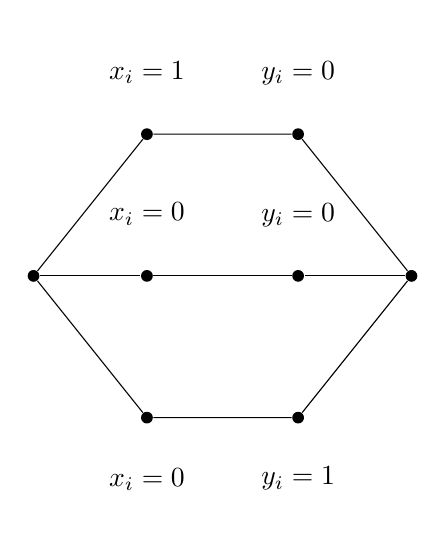
\begin{tikzpicture}[scale=1.2, every node/.style={circle, fill=black, inner sep=1.5pt}]

% Nodes

\node (L) at (-2,0) {};
\node (T1) at (-0.8,1.5) {};
\node (T2) at (0.8,1.5) {};
\node (M1) at (-0.8,0) {};
\node (M2) at (0.8,0) {};
\node (B1) at (-0.8,-1.5) {};
\node (B2) at (0.8,-1.5) {};
\node (R) at (2,0) {};

% Edges
\draw (L) -- (T1);
\draw (T1) -- (T2);
\draw (T2) -- (R);

\draw (L) -- (B1);
\draw (B1) -- (B2);
\draw (B2) -- (R);

\draw (L) -- (M1);
\draw (M1) -- (M2);
\draw (M2) -- (R);

% Labels
\node[draw=none, fill=none, above=6pt] at (T1) {$x_i = 1$};
\node[draw=none, fill=none, above=6pt] at (T2) {$y_i = 0$};

\node[draw=none, fill=none, above=6pt] at (M1) {$x_i = 0$};
\node[draw=none, fill=none, above=6pt] at (M2) {$y_i = 0$};


\node[draw=none, fill=none, below=6pt] at (B1) {$x_i = 0$};
\node[draw=none, fill=none, below=6pt] at (B2) {$y_i = 1$};

\end{tikzpicture}
\label{fig:disjoint_gadget}
\caption{Gadget for proving equality, a path only exists if $x_i$ and $y_i$ do not have the same element}
\end{figure}

\paragraph{Reduction to our graph problem.}
We construct a graph by chaining one copy of this gadget for each index $i \in [n]$ between a global start vertex $v$ and end vertex $w$. In the resulting graph, there exists a path from $v$ to $w$ if and only if all gadgets are traversable, which occurs if and only if $x$ and $y$ does not contain the same element\\


\begin{figure}[h]
\centering
\begin{tikzpicture}[
hex/.style={
draw,
regular polygon,
regular polygon sides=6,
minimum size=1.4cm,
inner sep=0pt
}
]

% Hexagons placed manually so edges touch
\node[hex] (h1) at (0,0) {};
\node[hex] (h2) at (1.4,0) {};
\node[hex] (h3) at (2.8,0) {};
\node[hex] (h4) at (4.2,0) {};
\node[hex] (h5) at (5.6,0) {};

% Draw horizontal line through the middle of all hexagons
\draw (-0.7,0) -- (6.3,0);

% Labels moved slightly up
\node[yshift=8pt] at (h1) {\scriptsize $i=1$};
\node[yshift=8pt] at (h2) {\scriptsize $i=2$};
\node[yshift=8pt] at (h3) {\scriptsize $i=3$};
\node[yshift=8pt] at (h4) {\scriptsize $\cdots$};
\node[yshift=8pt] at (h5) {\scriptsize $i=n$};

\end{tikzpicture}


\caption{Equality gadgets chained as adjacent hexagonal modules.}
\end{figure}

Therefore, any protocol that solves the reachability problem on this graph can be used to solve the Disjoint problem. Since Disjoint requires $\Omega(n)$ deterministic communication, it follows that our graph problem also requires $\Omega(n)$ deterministic communication.
